% THIS IS SIGPROC-SP.TEX - VERSION 3.1
% WORKS WITH V3.2SP OF ACM_PROC_ARTICLE-SP.CLS
% APRIL 2009
%
% It is an example file showing how to use the 'acm_proc_article-sp.cls' V3.2SP
% LaTeX2e document class file for Conference Proceedings submissions.
% ----------------------------------------------------------------------------------------------------------------
% This .tex file (and associated .cls V3.2SP) *DOES NOT* produce:
%       1) The Permission Statement
%       2) The Conference (location) Info information
%       3) The Copyright Line with ACM data
%       4) Page numbering
% ---------------------------------------------------------------------------------------------------------------
% It is an example which *does* use the .bib file (from which the .bbl file
% is produced).
% REMEMBER HOWEVER: After having produced the .bbl file,
% and prior to final submission,
% you need to 'insert'  your .bbl file into your source .tex file so as to provide
% ONE 'self-contained' source file.
%
% Questions regarding SIGS should be sent to
% Adrienne Griscti ---> griscti@acm.org
%
% Questions/suggestions regarding the guidelines, .tex and .cls files, etc. to
% Gerald Murray ---> murray@hq.acm.org
%
% For tracking purposes - this is V3.1SP - APRIL 2009

% THIS IS SIGPROC-SP.TEX - VERSION 3.1
% WORKS WITH V3.2SP OF ACM_PROC_ARTICLE-SP.CLS
% APRIL 2009
%
% It is an example file showing how to use the 'acm_proc_article-sp.cls' V3.2SP
% LaTeX2e document class file for Conference Proceedings submissions.
% ----------------------------------------------------------------------------------------------------------------
% This .tex file (and associated .cls V3.2SP) *DOES NOT* produce:
%       1) The Permission Statement
%       2) The Conference (location) Info information
%       3) The Copyright Line with ACM data
%       4) Page numbering
% ---------------------------------------------------------------------------------------------------------------
% It is an example which *does* use the .bib file (from which the .bbl file
% is produced).
% REMEMBER HOWEVER: After having produced the .bbl file,
% and prior to final submission,
% you need to 'insert'  your .bbl file into your source .tex file so as to provide
% ONE 'self-contained' source file.
%
% Questions regarding SIGS should be sent to
% Adrienne Griscti ---> griscti@acm.org
%
% Questions/suggestions regarding the guidelines, .tex and .cls files, etc. to
% Gerald Murray ---> murray@hq.acm.org
%
% For tracking purposes - this is V3.1SP - APRIL 2009

\documentclass{acm_proc_article-sp}

\usepackage{url}
\usepackage{listings}
\usepackage{graphicx}
\usepackage{fixltx2e}
\usepackage{moreverb}
\usepackage{fancyvrb}
\usepackage{csvsimple}
\usepackage{amsmath}
%\linespread{2}
\begin{document}

\numberofauthors{2}
\author{
\alignauthor
Ivan Oropeza\\
       \affaddr{Dept. of Computer Science}\\
       \affaddr{University of Texas at Austin}\\
\alignauthor
William Xie\\
       \affaddr{Dept. of Computer Science}\\
       \affaddr{University of Texas at Austin}\\
}

\title{Hidden Markov Models vs. Maximum Entropy Markov Models}


\maketitle

\section{Introduction}
\label{sec:introduction}

Sequence labeling is a frequently done task across many disciplines. DNA sequencing, video semantic analysis, and part-of-speech tagging are just some of the examples where sequence labeling is being used.~\cite{dnaEx, videoEx, nlpEx}. The tagging task was traditionally done manual by inspection and proved to be a very time consuming and costly task. In natural language processing (NLP), part-of-speech (POS) or lexical category tagging is an important stepping-stone to solving more complex problems such as semantic analysis of sentences. The typical techniques applied to this problem are hidden Markov models (HMM), maximum entropy Markov models (MEMM), and conditional random fields (CRF)~\cite{nlpBook}. We want to explore HMM and MEMM, two directed graphical models that shares the Markov assumption, through implementation and compare and contrast the learning and predicting mechanisms behind them as well as their performances. This paper is structured in the following way: first we provide a brief description of the corpora used in this investigation. Then, we discuss some of the similarities and differences between HMMs and MEMMs. Next, we explain how the training process works specifically for POS tagging. Then, we describe our implementation and experimental setup and analysis the performance of HMMs vs MEMMs under similar circumstances.


\section{Datasets}
For this investigation we focus on two corpora: the Wall Street Journal (WSJ) corpus and the Brown corpus. The WSJ corpus is a collection of 2,499 articles collected in a span of three years from the Wall Street Journal newspaper. It has approximately 3 million words and was tagged by using statistically-based methods. This corpus has a total of 82 possible POS tags~\cite{wsjCorpus}. On the other hand, the Brown corpus is a manually tagged collection of 500 text documents sampled from 1961. It uses 36 POS tags and it is consolidated from various sources and from various topics such as fiction, press, and lore~\cite{wsjCorpus}.

These two corpora are chosen because they are standards of the field, making them easy to obtain and allow us to compare our results to the rest of the NLP literature. In addition, they represent different extremes in distributions of words. The range of topics for the WSJ corpus is relatively narrow and specialized, thus it is reasonable to expect that the word choice distribution in the articles to be narrower than other corpora. Using similar logic, we expect the Brown corpus to represent a more general distribution on word choice. Therefore, by using two contrasting corpora are able to gauge the performance of the models in a broader set of situations in which POS tagging is used.

\begin{figure}[ht]
 \begin{Verbatim}[frame=single,framesep=5mm]
\[ He/PRP \]
tried/VBD to/TO ignore/VB
\[ what/WP \]

\[ his/PRP\$ own/JJ common/JJ sense/NN \]
told/VBD
\[ him/PRP \]
,/, but/CC
\[ it/PRP \]

\[ was/VBD n't/RB possible/JJ \]
;/: ;/:
\[ her/PRP$ motives/NNS \]
were/VBD too/RB blatant/JJ ./.
\end{Verbatim}
\caption{Example sentence from the Brown Corpus~\cite{brownCorpus} \label{brownExample}}
\end{figure}

\section{HMM vs. MEMM}
\label{sec:comparison}

An HMM is generative model for the joint distribution of states (POS tags) and observations (words). The model is captured by two matrices, transitional probability matrix for state to state and emission probability matrix for state to observation. The state transition follows the Markov assumption. In other words, a the transitions between states is restricted to be dependent only on the immediate past~\cite{nlpBook}. On the other hand, MEMM extends a maximum entropy classifier. It is a discriminative model that captures the conditional probability of the current state given the observation and the previous state. Figure \ref{hmmVmemm} shows pictorially the difference between the models.

The MEMM, like the maximum entropy model it is based on, is a multinomial logistic regression for classification but it focuses on making the fewest number of assumptions about the training data. Furthermore, the HMM only uses two aspects of the problem: the transition probabilities for states $P( S_i | S_{i-1} )$ and emission probabilities for the current state and observation $P( O_i | S_i )$. MEMM, in contrast, integrates feature information from the observations in addition to the previous state knowledge in order to derive a more accurate prediction model. This is captured in a single transitional probability matrix. For example, capitalization is closely associated with proper nouns and specific suffixes, such as "-ed" and "-ing", tend to be associated with verbs. These rules are useful features that can help improve the accuracy of the POS tagger which are not captured in the HMM model. Moreover, this model can be augmented further to include features involving additional past states and past or future observations~\cite{nlpBook}. Finally, the typical algorithms used to find the most probable state sequence for HMM can be modified for MEMM without additional overhead~\cite{memmPaper}.

However, MEMM is susceptible to the "label bias problem". This issue generally arises in two forms. First, if a state, $S_i$, has a high probability of transitioning to $S_j$ (low entropy with the extreme case of probability from $S_i$ to $S_j$ being 1), the observation would be less influential during the decoding process. In POS tagging this occurs when a sequence of observations and the corresponding tags appears abnormally frequently in the training set. The other source of bias is during labeling phase. When an observation occurs infrequently in the training set leads to an inaccurate tag, the tags for subsequent observations are affected by the error as well. \cite{labelBiasProblem}

\begin{figure}[ht]
\centering
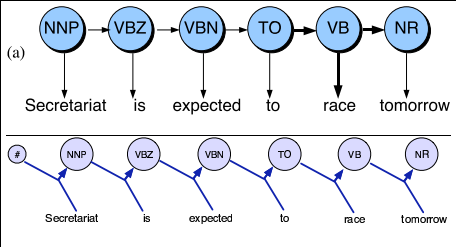
\includegraphics[width=80mm]{figures/memm.png}
\caption{(top) Hidden Markov Model and (bottom) Maximum Entropy Markov Model~\cite{nlpBook}. \label{hmmVmemm}}
\end{figure}

\section{Learning}
\label{sec:learning}
In POS tagging, training a HMM model in a supervised fashion reduces to a simple counting procedure~\cite{nlpBook}. In order to estimate $P( S_i | S_{i-1} )$ and $P( O_i | S_i )$, we can assume that our annotated corpus is a representative sample of the distribution we want to model, we can then define the distributions as follows:

\vspace{-1em}
\begin{equation}
P( S_i | S_{i-1} ) \approx \hat{P}( S_i | S_{i-1} ) = C( S_i, S_{i-1} )/C( S_{i-1} )
\end{equation}
\vspace{-1em}
\begin{equation}
P( O_i | S_i ) \approx \hat{P}( O_i | S_i ) = C( O_i, S_i )/C( S_i )
\end{equation}
where $\hat{P}$ is the probability with respect to the corpus and $C( O_i, S_i ), C( S_i, S_{i-1} )$, and $C( S_i )$ are the appropriate occurrences and co-occurrences of the observations and states.

However, there is one additional issue that needs to be addressed before the model can be used for tagging: how should the model respond to words that model did not encounter during training? If left unattended then $P( O_i | S_i ) = 0$ and consequently, Viterbi's algorithm will make incorrect decisions during the predicting process. The technique we employ to address this issue is Laplace smoothing (also known as additive smoothing)~\cite{laplaceSmooth}. The general idea of this approach is that every state will always have a small emission probability of producing an unseen word (denoted in our case by ``$\langle U \rangle $''). And every time the model encounters an unknown word it will use $P(\langle U \rangle| S )$ as the emission probability. The small probability is created by setting $C(\langle U \rangle, S ) = 1$ and incrementing $C( S )$ by 1 for each state $S$ after calculating the transition probabilities and before calculating the emission probabilities.

Training the MEMM is different from the straight forward counting method used in HMM. Since state transition depends on both previous state and the current observation, one large transition probability matrix (TPM) is employed. The TPM encapsulates all combinations of previous states $S_{i-1}$ and current observation $O_i$ pair in the training data to the current state $S_i$. Let $N$ represents the number of unique states and $M$ the number of unique words, the TPM has the shape $(N * M) \times N$. Each feature $f_a$ that we defined is an indicator function that takes $(O_i, S_{i-1})$ as arguments. An additional normalizing feature $f_x(O_i, S_i) = C - \sum\limits_{a} f_a(O_i, S_i)$ is added to ensure $(O, S)$ pairs not captured by specific features don't get penalized. The transitional probability takes the exponential family form:
\vspace{-1em}
\begin{equation}
P_{s_{i-1}}(S_i | O_i) = \frac{1}{Z(O_i, S_{i-1})} exp(\sum\limits_{a}\lambda_a f_a(O_i, S_i))
\end{equation}
where Z is the normalizing factor that makes the TPM sum to 1 across each row and $\lambda_a$ is the weight parameter that needs to be learned.

The training data is divided into $N$ buckets. For each sentence and for each $(word, tag)$ pair in it, the $(O_i, S_i)$ is placed the bucket corresponding to the $S_{i-1}$ tag. In other words, the training data is split into local training sets. This is different from HMM which treats the data globally. Let $m_{s_{i-1}}$ represent the number of observations per bucket. We then use generalized iterative scaling (GIS) algorithm to optimize each $\lambda_a$ to satisfy the following property for every tag $S_{i-1}$:

\vspace{-3em}
\begin{equation}
\begin{dmath}
\frac{1}{m_{s_{i-1}}}\sum\limits_{k=1}^{m_{s_{i-1}}} f_a(O_k, S_k) = \\ \frac{1}{m_{s_{i-1}}}\sum\limits_{k=1}^{m_{s_{i-1}}} \sum\limits_{S}P_{s_{i-1}}(S|O_k)f_a(O_k, S)
\end{dmath}
\end{equation}
\vspace{-5em}

where the left hand side is the average occurrence of the feature and the right hand side the expected value of the feature. We continuously update the $\lambda$'s and TPM until the expected value converges to the average. At this point, model is fully trained. The procedure is described in more detail in \cite{memmPaper}.

\section{Implementation and Results}
\label{sec:implementation}
We implemented both HMM and MEMM in Python using NumPy. For the HMM model, we leverage on the Viterbi algorithm provided by Hamilton~\cite{hmmCode} and the training was done as per section~\ref{sec:learning}. The following table shows the results for HMM when we execute our experiments using 20-fold cross-validation (train with 19 portions and test on 1). The HMM, due to its fast training, was trained using the entire corpus. In addition to evaluating performance on the testing data we also evaluated the model's performance on the training data. Testing the model with train data will give us an idea of over fitting (how much generalization is the model doing for this task) and testing with test data will give us an idea of the effectiveness of this model.
% HMM
\begin{figure}[ht]
  \begin{tabular}{ l || c | c | c | c | c }
    \bfseries & \bfseries & \bfseries \overline{Sentence} & \bfseries \sigma Sentence & \bfseries \overline{Tag} & \bfseries \sigma Tag

    \csvreader[head to column names]{figures/hmmScores.csv}{}% use head of csv as column names
    {\\\hline\csvcoli&\csvcolii&\csvcoliii&\csvcoliv&\csvcolv&\csvcolvi}% specify your coloumns here
    \end{tabular}
    \caption{HMM percent scores (\%) for the Brown and WSJ corpora. The first column is the corpus used. The second column is the data used for evaluating the system. Four scores are reported: the average and stdev for the number of sentences correctly tagged and the average and standard deviation for the number of tags correctly labled. \label{hmmScores}}
\end{figure}

The results show that the HMM parser performs significantly better with Brown in sentence accuracy than WSJ. Additionally, it also performs marginally better in tag accuracy. This contradicts our original hypothesis. For the sentence accuracy, this may be due to the length of the sentences. On average the Brown corpus has 16 observations per sentence. Meanwhile, WSJ has sentences averaging 53 observations. Another factor that may influence this score and the tag accuracy is the presence of unknown words. However, after further investigation, this hypothesis proved to be incorrect. On average Brown and WSJ encounter unknown words 12.1\% and 11.8\%. The data contradicts our hypothesis but the difference is marginal making the effect is inconclusive. Figure \ref{hmmScores1000} shows the results for the same experiment but limiting the number of sentences to 1000. Once again we see that Brown gives better performance (Figure ~\ref{fig:hmm1000}). We also attempted to shuffle the sentences before running the experiment in order mitigate problems related to domain adaptation, giving a more general result. As expected, the Brown corpus yields 93.7\% and 95.8\% for test and train data respectively and WSJ 91.5\% and 93.5\%.

%Another hypothesis that could explain these results is that because WSJ is targeted toward a demographic with high education background, its vocabulary might be broader. This makes the prediction more error prone when compared to a smaller vocabulary with higher concentration of common words.

\begin{figure}[ht]

  \begin{tabular}{ l || c | c | c | c | c }
    \bfseries & \bfseries & \bfseries \overline{Sentence} & \bfseries \sigma Sentence & \bfseries \overline{Tag} & \bfseries \sigma Tag

    \csvreader[head to column names]{figures/hmmScores@1000.csv}{}% use head of csv as column names
    {\\\hline\csvcoli&\csvcolii&\csvcoliii&\csvcoliv&\csvcolv&\csvcolvi}% specify your coloumns here
    \end{tabular}
    \caption{HMM percent scores (\%) for the Brown and WSJ corpora using only 1000 sentences.}
  \label{fig:hmm1000}
\end{figure}


On the other hand, we implemented MEMM entirely from scratch. The MEMM implementation is largely based on McCallum et al.'s algorithm for information extraction~\cite{memmPaper}. The training for MEMM is implemented based on the learning algorithm described in section~\ref{sec:learning}. The decoding algorithm we used is the modification on the Viterbi's algorithm described in~\cite{memmPaper}. Unknown words are handled using a uniform distribution in a similar fashion to Laplace smoothing for HMM. The condition for convergence is when the current value of $\lambda_a$ is within 0.1 of the previous value . The precision may be further improved at at the expense of computation time. Training with 1000 sentences from WSJ and Brown corpora, we acheived the sentence and tag accuracies are (0\%, 16.72\%) and (0\%, 20.67\%) respectively. The following table shows the results when we execute the same 20-fold experiment except we used total of 200 sentences.

%The following tables show the results for both models when we execute our experiments using 20-fold cross-validation (train with 19 portions and test on 1). In addition to evaluating performance on the testing data we also evaluated the model's performance on the training data. Testing the model with training data will give us an idea of over fitting (how much generalizable is the model for this task) and testing with testing data will give us an idea of effectiveness of the system.

% MEMM
\begin{figure}[ht]
  \begin{tabular}{ l || c | c | c | c | c }
    \bfseries & \bfseries & \bfseries \overline{Sentence} & \bfseries \sigma Sentence & \bfseries \overline{Tag} & \bfseries \sigma Tag

    \csvreader[head to column names]{figures/memmScores.csv}{}% use head of csv as column names
    {\\\hline\csvcoli&\csvcolii&\csvcoliii&\csvcoliv&\csvcolv&\csvcolvi}% specify your coloumns here
    \end{tabular}
    \caption{MEMM percent scores (\%) for the Brown and WSJ corpora using 200 sentences.}
\end{figure}

The results we obtained for MEMM are significantly lower than expected. With such low tag accuracy, 0\% sentence accuracy is a reasonable result. We believe this is the result of insufficient training data. The largest training set we were able to run was 1000 sentences. For WSJ and Brown, it generated TPM with dimensions $389,501 \times 49$ and $230,112 \times 48$ respectively, compared to the TPMs generated for 100 sentences $59,670 \times 39$ and $38,136 \times 42$. The computation time increases with the size of TPM making learning from large training data infeasible for the scope of this project given our GIS implementation. The 20-fold experiment took around 10 hours for each of the corpora. Moreover, because learning requires dividing observations into buckets, the problem amplifies. For example, if the observation ``THE'' with tag ``DT'' appears in the training data $c$ times, the occurrences would be divided among the previous state buckets for ``NN'', ``VB'', ``DT'', etc. Each bucket would have far fewer than the total $c$ occurrences, drawing inconclusive probabilities. Following this logic, MEMM benefits more in having a large training set than HMM. In addition, with the non-trivial chance of error due to small training set, the modified Viterbi's algorithm magnifies the problem by propagating the error through the sentence. Test set performed even worse due to the introduction of smoothing in addition to the aforementioned problems. Another reason for the cause of the low accuracy is the possibility of GIS converging to local maxima. We believe with more training data, the MEMM model could perform significantly better than it is currently performing.

Given the poor results from our implementation of MEMM, we have tested each part of the program individually and intensively by manually creating ideal data, transitional probabilities, and other features of the model. Through inspection, each part seems to be behave as expected and no bugs was found. Even though the accuracy of the experiments is low, it is still in line with the performance of HMM with Brown having higher tag accuracy than WSJ. This leads us to believe the main culprit remains to be the small training set.

Given that our implementation of MEMM performs considerably worse than expected due to the insufficent training data, we cannot draw meaningful conclusions based on the results. Ideally, we would compare not only the overall performance of the models but also determine which POS tags experience an increase in accuracy.

Nevertheless, the literature shows that MEMM tends to outperform HMM in POS tagging. Brants reports that their HMM POS tagger reaches 96.46\% accuracy in the WSJ corpus while Denis and Sagot's MEMM tagger correctly tags 96.96\% for the same corpus. ~\cite{memmAhmmResultsACL}. Figure~\ref{allScores} shows the results for various experiments in POS tagging.

\begin{figure}[ht]
  \begin{tabular}{ l | c | c | c | c | r }
    \bfseries Corpus & \bfseries Model & \bfseries Accuracy & \bfseries Authors

    \csvreader[head to column names]{figures/otherResults.csv}{}% use head of csv as column names
    {\\\hline\csvcoli&\csvcolii&\csvcoliii&\csvcoliv}% specify your coloumns here
    \end{tabular}
    \caption{Accuracy results for various POS tagging experiments. \label{allScores}}
\end{figure}
\section{Conclusion}
We have explored two graphical models, HMM and MEMM, in the POS tagging application domain. Through implementation of both models, we gained deeper understanding for the learning and predicting mechanisms behind each model and how to realize them from data parsing, to constructing the models, and lastly learn and predict using them. We ran both models through the Brown and WSJ corpora, we were able get satisfactory results for HMM but not MEMM. This is mainly due to the insufficient training data and the relatively long time compared to HMM to train it. During the implementation process, we learned that smoothing is a key feature to have for both models to produce meaningful prediction results, even rudimentary additive smoothing is powerful enough to produce viable results.

HMM and MEMM are just two of numerous models used for POS tagging. Even though both look similar on the surface, the implementation of the learning proved to be drastically different. For future work, in addition to training the model with more data and apply additional optimization techniques, we hope to extend MEMM to incorporate more features, especially more sophisticated ones that involves more than one state or observation, to see performance differences.

Overall, we find project to be an invaluable learning experience to be
exposed to strengths and weaknesses of graphical models by implementation and an important stepping-stone to understanding and implementing more sophisticated graphical models.


\bibliographystyle{abbrv}
\bibliography{references}
\end{document}
